\documentclass{report}
\usepackage[utf8]{inputenc}
\usepackage{amsmath}
\usepackage{graphicx}
\usepackage{amsfonts}
\usepackage{amssymb}

\title{Eksamensnoter - Amortized Analysis}
\author{André Oskar Andersen (wpr684)}
\date{\today}

\begin{document}
\maketitle

\section*{25 Single-Source Shortest Paths}
\begin{itemize}
    \item In a \textit{shortest-paths problem}, we are given a weighted, directed graph $G = (V, E)$, with weight function $w: E \rightarrow \mathbb{R}$ mapping edges to real-valued weights. The \textit{weight} $w(p)$ of path $p = \{v_0, v_1, ..., v_k\}$ is the sum of the weights of its constituent edges:
    $$w(p) = \sum^k _{i = 1} w(v_{i - 1}, v_i)$$
    \item We define the \textit{shortest-path weight} $\delta(u, v)$ from $u$ to $v$ by
    \[
      \delta(u, v) =
      \begin{cases}
          \min\{w(p): u \rightsquigarrow^p v\} & \text{if there is a path from $u$ to $v$} \\
          \infty & \text{otherwise}
      \end{cases}
    \]
    A \textit{shortest path} from vetex $u$ to vertex $v$ is then defined as any path $p$ with weight $w(p) = \delta(u, v)$
\end{itemize}
\textbf{Variants}
\begin{itemize}
    \item In the \textit{single-source shortest-paths problem} we are given a graph $G = (V, E)$ and we want to find a shortest path from a given \textit{source} vertex $s \in V$ to each vertex $v \in V$
    \item In a \textit{single-destination shortest-paths problem} the goal is to find a shortest path to a given \textit{destination} vertex $t$ from each vertex $v$. 
    \item In a \textit{single-pair shortest-path problem} the goal is to find a shortest path from $u$ to $v$ for given vertices $u$ and $v$.
    \item In a \textit{all-pair shortest-paths problem} the goal is to find a shortest path from $u$ to $v$ for every pair of vertices $u$ and $v$. Although we can sole this problem by running a single-source algorithm once from each vertex, we usually can solve it faster
\end{itemize}
\textbf{Optimal substructure of a shortest path}
\begin{itemize}
    \item Shortest-paths algorithms typically rely on the property that a shortest path between two vertices contains other shortest paths within it
    \item The following lemma states the optimal-substructure property of shortest paths more precisely: \\
    \textbf{Lemma 24.1 (Subpaths of shortest paths are shortest paths)}:
    \begin{itemize}
        \item Given a weighted, directed graph $G = (V, E)$ with weight function $w: E \rightarrow \mathbb{R}$, let $p = \{v_0, v_1, ..., v_k\}$ be a shortest path from vertex $v_0$ vertex $v_k$ and, for any $i$ and $j$ such that $0 \leq i \leq j \leq k$, let $p_{ij} = \{v_i, v_{i + 1}, ..., v_j\}$ be the subpath of $p$ from vertex $v_i$ to vertex $v_j$. Then, $p_{ij}$ is a shortest path from $v_i$ to $v_j$.
    \end{itemize}
\end{itemize}
\textbf{Negative-weight edges}
\begin{itemize}
    \item Some isntances of the single-source shortest-paths problem may include edges whose weights are negative. If there is a negative-weight cycle on some path from $s$ to $v$, we define $\delta(s, v) = -\infty$
    \item Dijkstra's algorithm assume that alle edge weights in the input graph are nonnegative. The Bellman-Ford algorithm allow negative-weight edges in the input graph and produce a correct answer as long as no negative-weight cycles are reachable from the source. Typically, if there is such a negative-weight cycle, the algorithm can detect and report its existence
\end{itemize}
\textbf{Cycles}
\begin{itemize}
    \item Without loss of generality we can assume that when we are finding shortest paths, they have no cycles, i.e., they are simple paths.
\end{itemize}
\textbf{Representing shortest paths}
\begin{itemize}
    \item We often wish to compute not only shortest-path weights, but the vertices on shortest paths as well
    \item Given a graph $G = (V, E)$, we maintain for each vertex $v \in V$ as \textit{predecessor} $v.\pi$ that is either another vertex or \texttt{NIL}
    \item In the mdst of executing a shortest-paths algorithm, howeever, the $\pi$ values might not indicate shortest paths. We shall be interested in the \textit{predecessor subgraph} $G_{\pi} = (V_{\pi}, E_{\pi})$ induced by the $\pi$ values. Here we define the vertex set $V_{\pi}$ to be the set of vertices $G$ with non-\texttt{NIL} predecessors, plus the source $s$:
    $$V_{\pi} = \{v \in V: v.\pi \neq \texttt{NIL}\} \cup \{s\}$$
    The directed edge set $E_{\pi}$ is the set of edges induced by the $\pi$ values for vertices in $V_{\pi}$:
    $$E_{\pi} = \{(v.\pi, v) \in E: v \in V_{\pi} - \{s\}\}$$
    \item A \textit{shortest-paths tree} rooted at $s$ is a directed subgraph $G' = (V', E')$, where $V' \subset V$ and $E' \subset E$ such that
    \begin{enumerate}
        \item $V'$ is the set of vertices reachable from $s$ in $G$
        \item $G'$ forms a rooted tree with root $s$
        \item for all $v \in V'$, the unique simple path from $s$ to $v$ in $G'$ is a shortest path from $s$ to $v$ in $G$
    \end{enumerate}
\end{itemize}
\textbf{Relaxation}
\begin{center}
    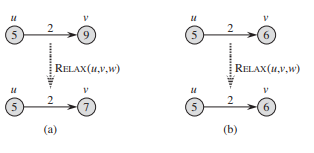
\includegraphics[width = 6 cm]{../entities/relaxing.png}
\end{center}
\begin{itemize}
    \item For each vertex $v \in V$, we maintai nan attribute $v.d$ which is an upper bound on the weight of a shortest path from source $s$ to $v$. We call $v.d$ a \textit{shortest-path estimate}
    \item Afer initialization, we have $v.\pi = \texttt{NIL}$ for all $v \in V$, $s.d = 0$, and $v.d = \infty$ for $v \in V - \{s\}$
    \item The process of \textit{relaxing} an edge $(u, v)$ consists of testing whether we can improve the shortest path to $v$ found so far by going through $u$ and, if so, updating $v.d$ and $v.\pi$.
\end{itemize}
\textbf{Properties of shortest paths and relaxation}
\begin{itemize}
    \item \textit{Triangle inequality}: For any edge $(u, v) \in E$ we have $\delta(s, v) \leq \delta(s, u) + w(u, v)$
    \item \textit{Upper-bound property}: We always have $v.d \geq \delta(s, v)$ for all vertices $v \in V$, and once $v.d$ achieves the value $\delta(s, v)$, it never changes
    \item \textit{No-path property}: If there is not path from $s$ to $v$, then we always have $v.d = \delta(s, v) = \infty$
    \item \textit{Convergence property}: If $s \rightsquigarrow u \rightarrow$ is a shortest path in $G$ for some $u, v \in V$, and if $u.d = \delta(s, u)$ at any time prior to relaxing edge $(u, v)$, then $v.d = \delta(s, v)$ at all time afterward
    \item \textit{Path-relaxation property}: If $p = \{v_0, v_1, ..., v_k\}$ is a shortest path from $s = v_0$ to $v_k$, aand we relax the edges of $p$ in order $(v_0, v_1), (v_1, v_2), ..., (v_{k - 1}, v_k)$, then $v_k.d = \delta(s, v_k)$.
    \item \textit{Predecessor-subgraph property}: Once $v.d = \delta(s, v)$ for all $v \in V)$, the predecessor subgraph is a shortest-paths tree rooted at $s$
\end{itemize}
\subsection*{24.1 The Bellman-Ford algorithm}
\begin{center}
    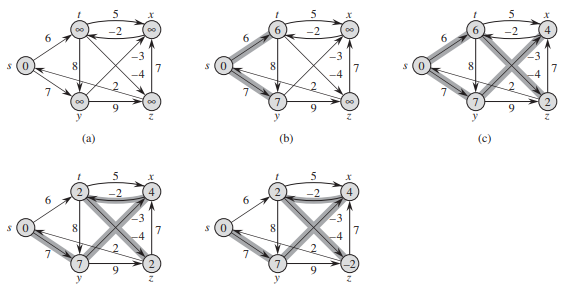
\includegraphics[width = 8 cm]{../entities/bellman_ford.png}
\end{center}
\begin{itemize}
    \item The \textit{Bellman-Ford algorithm} solves the single-source shortest-paths problem in general case in which edge weights may be negative.
    \item Given a weighted, directed graph with source $s$ and weight function $w$, the Bellman-Ford algorithm returns a boolean value indicating whether or not there is a negative-weight cycle that is reachable from the source. If there is such a cycle, the algorithm indicates that no solution exists. If there is no such cycle, the algorithm produces the shortst paths and their weights 
    \item The Bellman-Ford algorithm runs in time $O(VE)$
\end{itemize}
\subsection*{24.3 Dijkstra's algorithm}
\begin{center}
    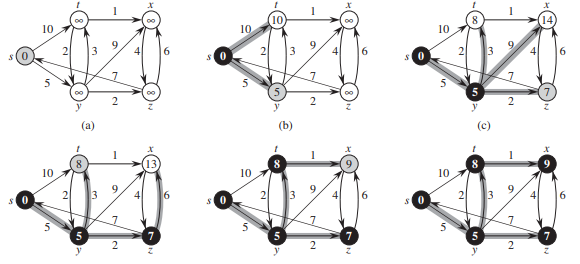
\includegraphics[width = 8 cm]{../entities/dijkstra.png}
\end{center}
\begin{itemize}
    \item Dijkstra's algorithm solves the single-source shortest-paths problem on a weighted, directed graph for the case in which all edge weights are nonnegative.
    \item Dijktra's algorithm maintains a set $S$ of vertices whose final shortest-path weights from the source $s$ have already been determined. The algorithm repeatedly selects the vertex $u \in V - S$ with the minimum shortest-path estimate, adds $u$ to $S$, and relaxes all edges leaving $u$.
    \item The total running is $O((V + E) \lg V)$, which is $O(E \lg V)$ if all vertices are reachable from the source. We can achieve a running time of $O(V \lg V + E)$ by implementing the min-priority queue with a Fibonacci heap.
\end{itemize}

\section*{25 All-Pairs Shortest Paths}
\begin{itemize}
    \item In this chapter, we consider the problem of finding shortest paths between all pairs of vertices in a graph.
    \item We typically want the output in tabular form: the endtries in $u$'s row and $v$'s column should be the weight of a shortest path from $u$ to $v$
    \item We assume that the vertices are numbered $1, 2, ..., |V|$, so that the input is an $n \times n$ matrix $W$ representing the edge weights of an $n$-vertex directed graph. That is, $W = (w_{ij})$, where
    \[
    w_{ij} = 
    \begin{cases}
        0 & \text{if $i = j$} \\
        \text{the weight of directed edge $(i, j)$} & \text{if $i \neq j$ and $(i, j) \in E$} \\
        \infty & \text{if $i \neq j$ and $(i, j) \notin E$} \\
    \end{cases}    
    \]
    \item We allow negative-weight edges, but we assume for the time being that the input graph contains no negative-weight cycles
    \item To solve the all-pair shortest-paths prolem on an input adjacency matrix, we need to compute not only the hosrtest-path weights but also a \textit{predecessor matrix} $\prod = (\pi_{ij})$, where $\pi_{ij}$ is \texttt{NIL} if either $i = j$ or there is not path from $i$ to $j$, and otherweise $\pi_{ij}$ is the predecessor of $j$ on some shortest path from $i$. The subgraph induced by the $i$th row of the $\prod$ matrix should be a shortest-paths tree with root $i$. For each vertex $i \in V$, we define the \textit{predecessor subgraph} of $G$ for $i$ as $G_{\pi, i} = (V_{\pi, i}, E_{\pi, i})$, where
    $$V_{\pi, i} = \{j \in V: \pi_{ij} \neq \texttt{NIL}\} \cup \{i\}$$
    and
    $$E_{\pi, i} = \{(\pi_{ij}, j): j \in V_{\pi, i} - \{i\}\}$$
\end{itemize}
\end{document}